\chapter{Metodologia}

Este capítulo aborda o planejamento e execução do projeto, contendo os procedimentos e técnicas utilizadas, possibilitando a sua  replicação. Tendo em vista os conceitos descritos no capítulo \ref{cha:pln} (Processamento de Linguagem Natural), o presente trabalho tem como objetivo responder à seguinte questão problema:

\begin{center}
\textit{É possível extrair o perfil temático dos deputados através da análise dos seus discursos e proposições utilizando técnicas clássicas de aprendizado de máquina e processamento de linguagem natural?}
\end{center}

Além disso, será construído um \textit{web site} com o intuito de fornecer uma forma melhor de visualização dos dados obtidos nesta análise, através de gráficos interativos que garantam que o usuário tenha uma boa experiência de usabilidade.

\section{Trabalhos Relacionados}

Durante a pesquisa bibliográfica realizada neste trabalho, encontrou-se alguns trabalhos que também fizeram análise de textos parlamentares utilizando aprendizado bayesiano. O Retórica Parlamentar\footnote{http://retorica.labhackercd.net/about.html}, idealizado por Davi Moreira\footnote{https://github.com/davi-moreira}, Manoel Galdino\footnote{https://github.com/mgaldino} e Luis Carli\footnote{https://github.com/luiscarli}, utiliza os discursos proferidos pelos parlamentares no Pequeno Expediente e no Grande Expediente da Câmara dos Deputados para promover a transparência do mandato e fornecer subsídios para o controle social com a divulgação dos temas mais debatidos em Plenário.

A técnica utilizada pelo Retórica para a classificação dos discursos é um modelo bayesiano hierárquico, descrito por \citeonline{grimmer2009}, onde através de aprendizado não supervisionado são gerados \(k\) \textit{clusters}, sendo \(k\) um valor escolhido ao executar o algoritmo. O resultado é exportado para o formato \textit{csv} e contém os termos mais frequentes de cada cluster. Em seguida, um especialista deve ler e rotular cada \textit{cluster}.

A visualização dos dados é feita através de um gráfico de bolhas, em que cada bolha representa a relevância (medida pela frequência) de cada tema dentre todos os deputados analisados. Dentro de cada bolha são colocados os deputados que enfatizam aquele tema nos seus discursos. Um deputado está associado a um único tema, que é o tema mais enfatizado por ele nos seus discursos.

\begin{figure}[h]
    \centering
    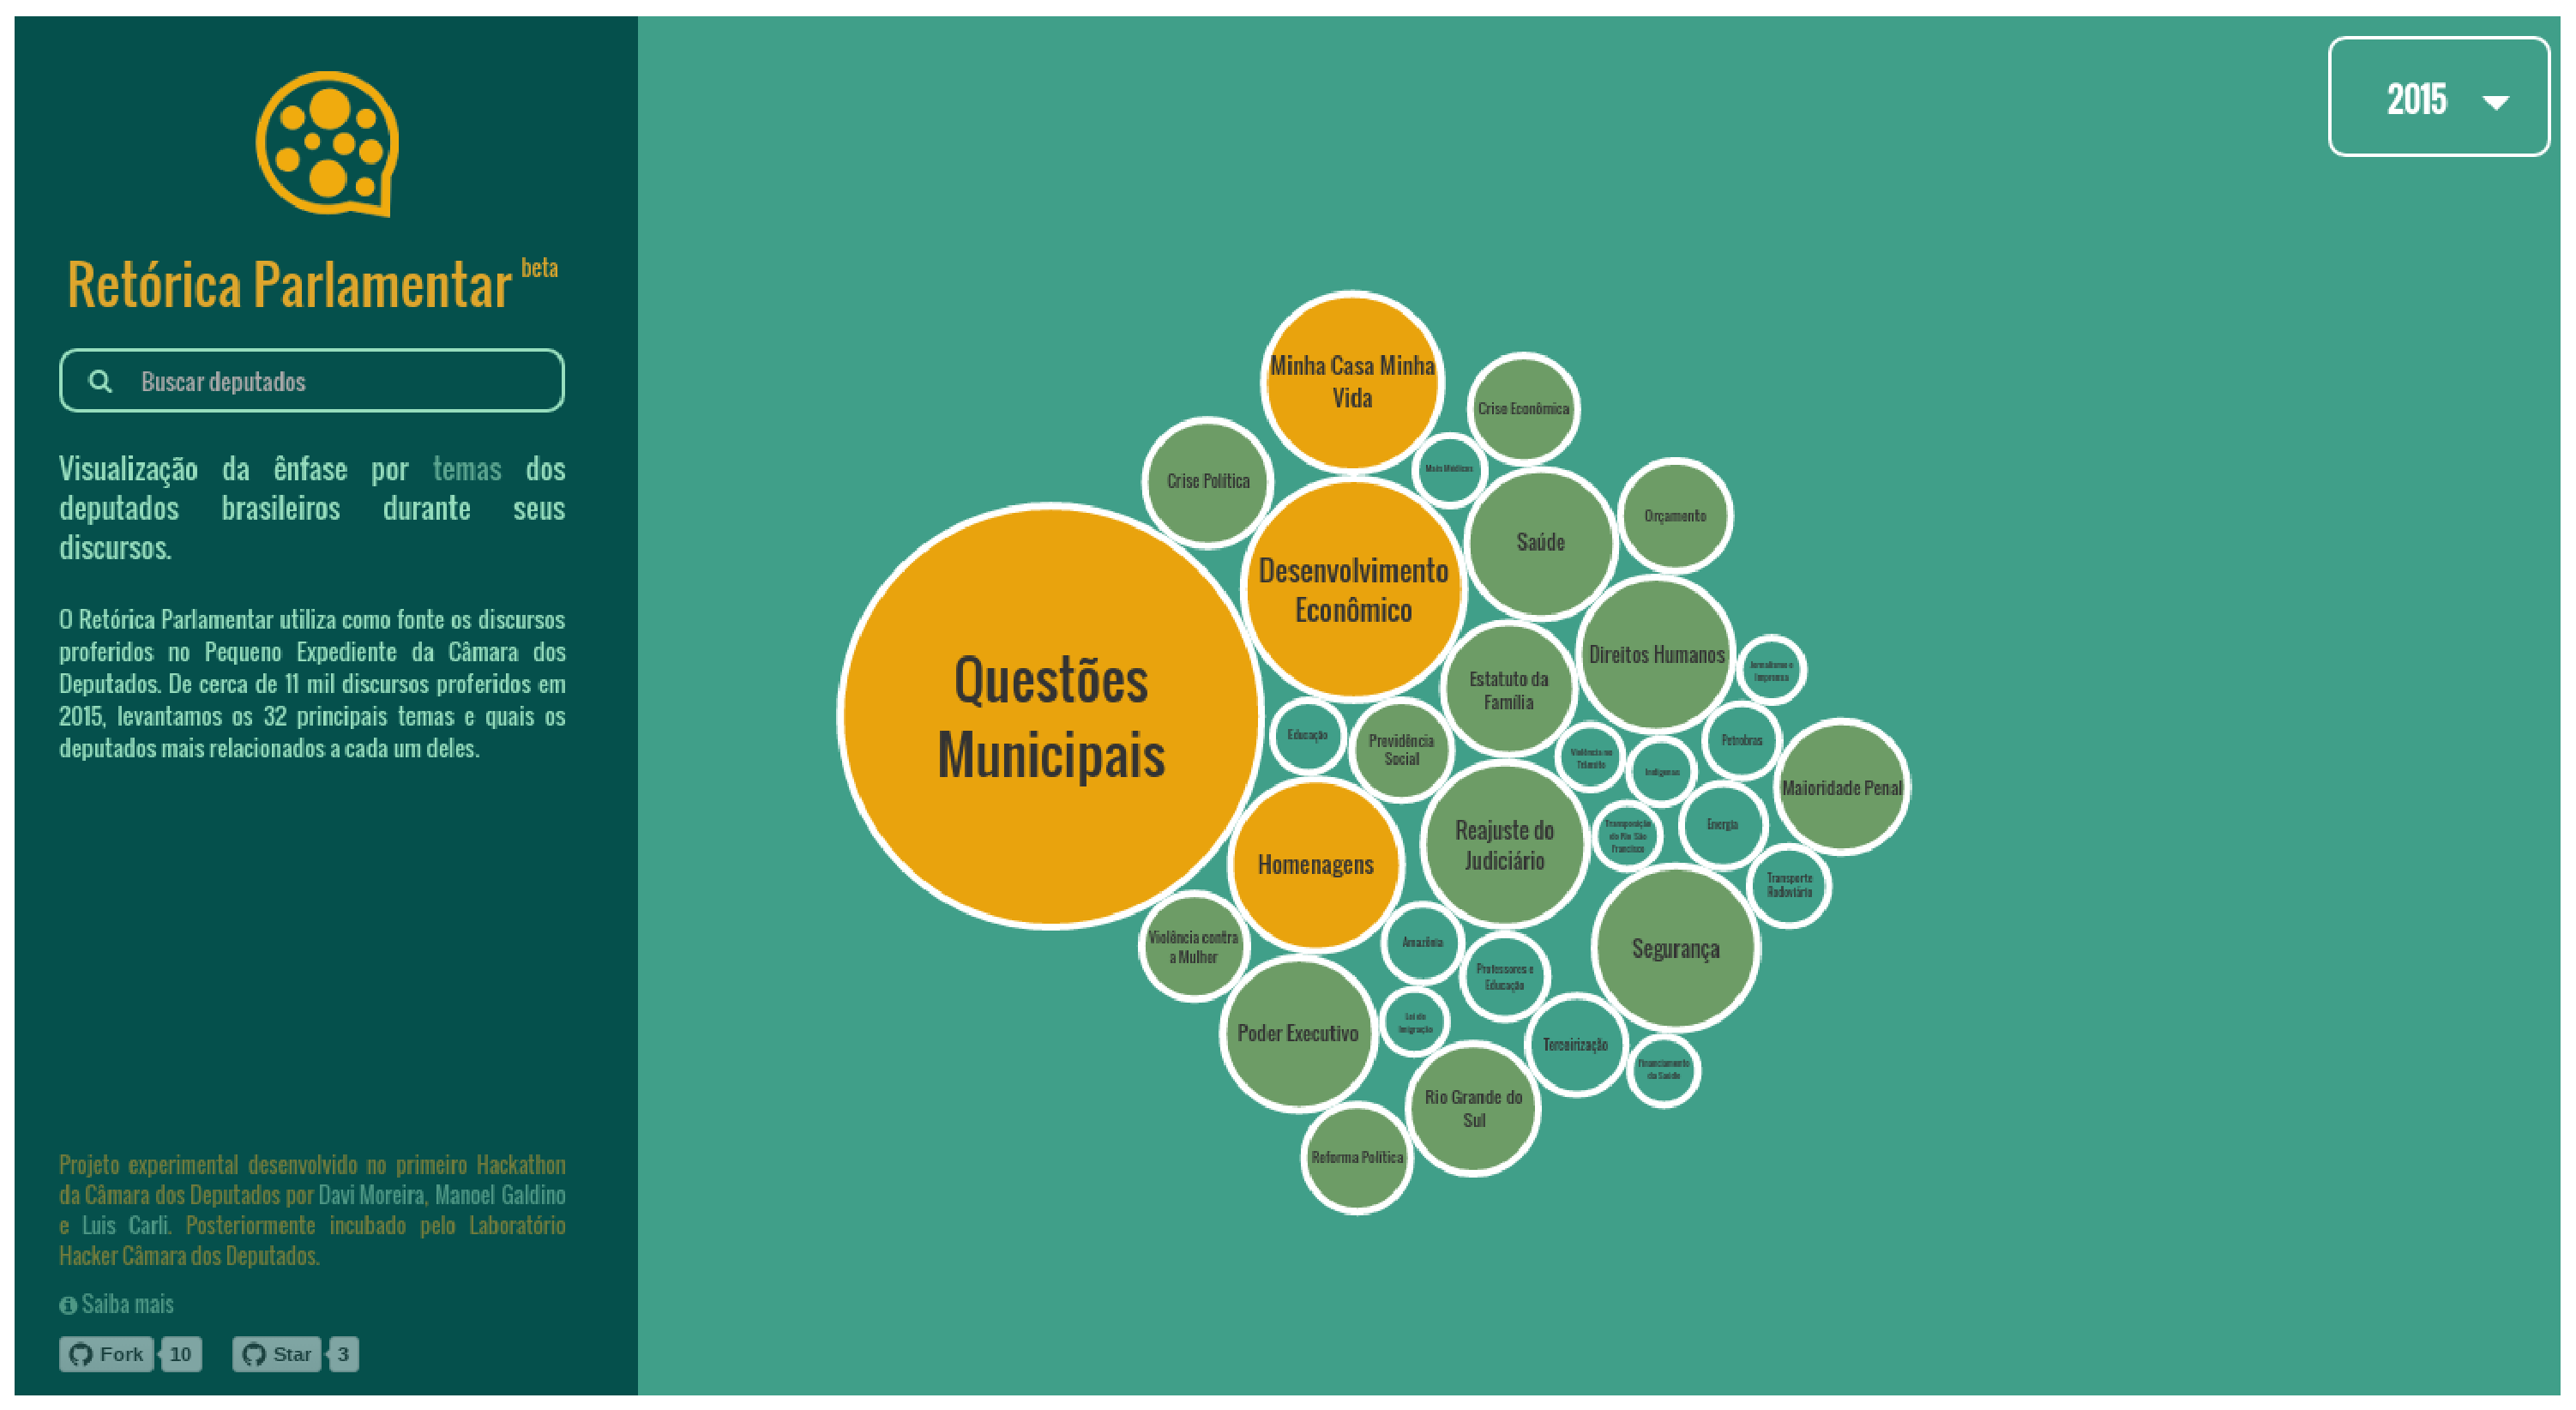
\includegraphics[scale=0.3]{figuras/retorica.eps}
    \caption{Retórica Parlamentar}
\end{figure}

\section{Planejamento das Atividades}

Para a realização desse trabalho, foram identificadas algumas atividades que seguem um fluxo de trabalho previsível, como mostra o diagrama a seguir:

As atividades realizadas

\begin{figure}[h]
    \centering
    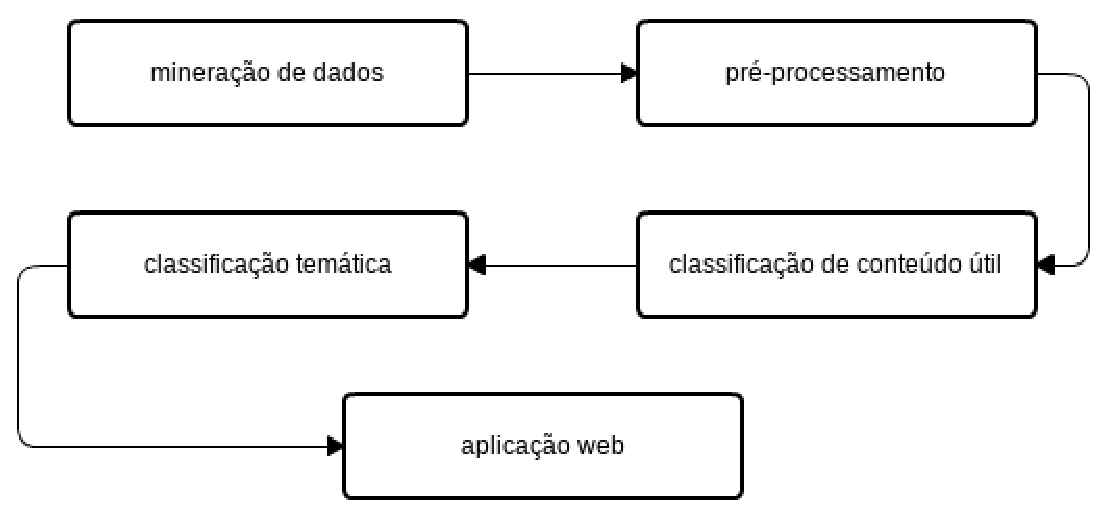
\includegraphics[scale=0.5]{figuras/planejamento.eps}
    \caption{Diagrama de planejamento}
\end{figure}

As seções seguintes descrevem cada etapa apresentada acima.

\subsection{Mineração de Dados}

A obtenção e persistência dos dados será realizada por uma biblioteca desenvolvida pelo autor, descrita na seção \ref{obtencao-dados} e consiste em realizar consultas ao \textit{webservice} da Câmara dos Deputados, fazendo um processamento inicial, afim de padronizar as informações e transformá-las em seus tipos correspondentes na linguagem \textit{Python}. Os dados provenientes do \textit{webservice} estão em formato \textit{XML} e armazenam valores como \textit{strings}.

Nesta etapa transformamos todos os campos com valores de números inteiros e decimais, datas, horários e textos em, respectivamente, valores \textit{Python} correspondentes. Além disso, também é realizada a persistência dessas informações em banco de dados relacional.

\subsection{Pré-processamento}

Apesar do ``pré-processamento'' não depender tanto dos dados reais, a definição das \textit{stop words} deve ser feita levando em consideração o conteúdo que será analisado.

A etapa de pré-processamento consiste na análise dos textos obtidos na mineração de dados, afim de identificar as \textit{stop words} presentes em textos do contexto legislativo. Além disso, deve ser realizada o processo de \textit{stemização} para reduzir a dimensionalidade das \textit{bag-of-words} geradas.

Estudamos diferentes estratégias para a utilização de \(n\)-gramas, mas por enquanto decidiu-se, por uma questão de simplicidade, limitar-se apenas ao uso de unigramas.

\subsection{Classificação Conteúdo Útil}

Essa classificação tem como objetivo melhorar a qualidade da análise temática dos deputados. Uma parte considerável dos textos não possuem valor semântico significativo, pois tratam de questões protocolares e de trâmite legislativo. Citamos um exemplo: \textit{``É preciso haver quórum de 257 Srs. Deputados para aprovação da matéria, quórum mínimo. A votação é normal. Então, acho que, quando houver uns 300 ou 320 votos, encerraremos.''}. Portanto, a classificação entre conteúdo útil/não-útil consiste em separar os parágrafos que realmente possuem valor para a análise posterior dos que não devem ser usados nestas análises.

Essa atividade não foi mais adotada para a segunda parte desse trabalho, pois optou-se pela não utilização dos textos completos dos discursos, substituindo-os pelos sumários e indexações. Com essa nova abordagem, a análise é feita utilizando um resumo (sumário) do discurso, onde cada frase, geralmente, representa um tema abordado pelo parlamentar. Também foi utilizado um conjunto de palavras que são utilizadas para a busca no próprio site da Câmara dos Deputados. Tanto os sumários quanto as indexação são elaborados por um departamento da Casa, por profissionais especializados em Arquitetura da Informação.

\subsection{Classificação Temática}

Após determinar quais parágrafos serão análisados, os mesmos devem ser classificados de acordo com alguns temas. Para o contexto do TCC 1, foram selecionados inicialmente: Agropecuária, Saúde, Esporte, Educação, Ciência e Tecnologia, Economia, Política, Meio Ambiente, Direitos Humanos e Segurança. Para a realização dessa tarefa, foi necessário construir um texto inicial para cada um dos temas listados, afim de fornecer um parâmetro inicial ao classificador. Os textos iniciais de cada tema têm como base textos previamente classificados em portais de notícias brasileiros e consistem em apenas uma listagem de palavras comuns relacionadas a estes temas.

Para o TCC 2, a base inicial de palavras foi obtida através do Tesauro da Câmara dos Deputados, que possui uma base de 14611 termos, agrupados em 49 áreas temáticas. Tal agrupamento foi realizado por profissionais da área de arquitetura da informação da própria Câmara.

54 temas é uma quantidade relativamente grande, o que poderia dificultar um pouco a análise. Foi realizado um agrupamento dessas áreas temáticas e reduzidos para 22 temas. As tabelas a seguir mostra todos os temas e seus agrupamentos (macro-temas):

\begin{table}[h]
\centering
\begin{tabular}{clc}
\hline
\multicolumn{1}{|c|}{\textbf{\begin{tabular}[c]{@{}c@{}}Quantidade\\ de Termos\end{tabular}}} & \multicolumn{1}{c|}{\textbf{Tema}} & \multicolumn{1}{c|}{\textbf{Macro-tema}} \\ \hline
\multicolumn{1}{|c|}{57} & \multicolumn{1}{l|}{Administração} & \multicolumn{1}{c|}{Gestão} \\ \hline
\rowcolor[HTML]{EFEFEF}
\multicolumn{1}{|c|}{\cellcolor[HTML]{EFEFEF}1481} & \multicolumn{1}{l|}{\cellcolor[HTML]{EFEFEF}Administração Pública} & \multicolumn{1}{c|}{\cellcolor[HTML]{EFEFEF}Administração Pública} \\ \hline
\multicolumn{1}{|c|}{304} & \multicolumn{1}{l|}{Agricultura, Pecuária e Pesca} & \multicolumn{1}{c|}{} \\ \cline{1-2}
\multicolumn{1}{|c|}{78} & \multicolumn{1}{l|}{Política Fundiária} & \multicolumn{1}{c|}{\multirow{-2}{*}{Agricultura, Pecuária e Pesca}} \\ \hline
\rowcolor[HTML]{EFEFEF}
\multicolumn{1}{|c|}{\cellcolor[HTML]{EFEFEF}{\color[HTML]{000000} 97}} & \multicolumn{1}{l|}{\cellcolor[HTML]{EFEFEF}{\color[HTML]{000000} Ciência da Informação}} & \multicolumn{1}{c|}{\cellcolor[HTML]{EFEFEF}} \\ \cline{1-2}
\rowcolor[HTML]{EFEFEF}
\multicolumn{1}{|c|}{\cellcolor[HTML]{EFEFEF}{\color[HTML]{000000} 221}} & \multicolumn{1}{l|}{\cellcolor[HTML]{EFEFEF}{\color[HTML]{000000} Arte e Cultura}} & \multicolumn{1}{c|}{\cellcolor[HTML]{EFEFEF}} \\ \cline{1-2}
\rowcolor[HTML]{EFEFEF}
\multicolumn{1}{|c|}{\cellcolor[HTML]{EFEFEF}{\color[HTML]{000000} 17}} & \multicolumn{1}{l|}{\cellcolor[HTML]{EFEFEF}{\color[HTML]{000000} Artes e Letras}} & \multicolumn{1}{c|}{\multirow{-3}{*}{\cellcolor[HTML]{EFEFEF}Artes, Cultura e Informação}} \\ \hline
\multicolumn{1}{|c|}{180} & \multicolumn{1}{l|}{Ciência e Tecnologia} & \multicolumn{1}{c|}{} \\ \cline{1-2}
\multicolumn{1}{|c|}{192} & \multicolumn{1}{l|}{Informática e TI} & \multicolumn{1}{c|}{} \\ \cline{1-2}
\multicolumn{1}{|c|}{264} & \multicolumn{1}{l|}{Comunicações} & \multicolumn{1}{c|}{\multirow{-3}{*}{Ciência e Tecnologia}} \\ \hline
\rowcolor[HTML]{EFEFEF}
\multicolumn{1}{|c|}{\cellcolor[HTML]{EFEFEF}45} & \multicolumn{1}{l|}{\cellcolor[HTML]{EFEFEF}Comércio Exterior} & \multicolumn{1}{c|}{\cellcolor[HTML]{EFEFEF}} \\ \cline{1-2}
\rowcolor[HTML]{EFEFEF}
\multicolumn{1}{|c|}{\cellcolor[HTML]{EFEFEF}132} & \multicolumn{1}{l|}{\cellcolor[HTML]{EFEFEF}Relações Internacionais} & \multicolumn{1}{c|}{\multirow{-2}{*}{\cellcolor[HTML]{EFEFEF}Relações Exteriores}} \\ \hline
\multicolumn{1}{|c|}{36} & \multicolumn{1}{l|}{Comunicação Social} & \multicolumn{1}{c|}{Comunicação Social} \\ \hline
\rowcolor[HTML]{EFEFEF}
\multicolumn{1}{|c|}{\cellcolor[HTML]{EFEFEF}139} & \multicolumn{1}{l|}{\cellcolor[HTML]{EFEFEF}Economia} & \multicolumn{1}{c|}{\cellcolor[HTML]{EFEFEF}} \\ \cline{1-2}
\rowcolor[HTML]{EFEFEF}
\multicolumn{1}{|c|}{\cellcolor[HTML]{EFEFEF}45} & \multicolumn{1}{l|}{\cellcolor[HTML]{EFEFEF}Contabilidade} & \multicolumn{1}{c|}{\cellcolor[HTML]{EFEFEF}} \\ \cline{1-2}
\rowcolor[HTML]{EFEFEF}
\multicolumn{1}{|c|}{\cellcolor[HTML]{EFEFEF}281} & \multicolumn{1}{l|}{\cellcolor[HTML]{EFEFEF}Finanças Públicas e Orçamento} & \multicolumn{1}{c|}{\cellcolor[HTML]{EFEFEF}} \\ \cline{1-2}
\rowcolor[HTML]{EFEFEF}
\multicolumn{1}{|c|}{\cellcolor[HTML]{EFEFEF}38} & \multicolumn{1}{l|}{\cellcolor[HTML]{EFEFEF}Política Econômica} & \multicolumn{1}{c|}{\cellcolor[HTML]{EFEFEF}} \\ \cline{1-2}
\rowcolor[HTML]{EFEFEF}
\multicolumn{1}{|c|}{\cellcolor[HTML]{EFEFEF}282} & \multicolumn{1}{l|}{\cellcolor[HTML]{EFEFEF}Sistema Financeiro} & \multicolumn{1}{c|}{\cellcolor[HTML]{EFEFEF}} \\ \cline{1-2}
\rowcolor[HTML]{EFEFEF}
\multicolumn{1}{|c|}{\cellcolor[HTML]{EFEFEF}235} & \multicolumn{1}{l|}{\cellcolor[HTML]{EFEFEF}Tributação} & \multicolumn{1}{c|}{\multirow{-6}{*}{\cellcolor[HTML]{EFEFEF}Economia e Finanças Públicas}} \\ \hline
\multicolumn{1}{|c|}{27} & \multicolumn{1}{l|}{Desenvolvimento Regional} & \multicolumn{1}{c|}{Desenvolvimento Regional} \\ \hline
\rowcolor[HTML]{EFEFEF}
\multicolumn{1}{|c|}{\cellcolor[HTML]{EFEFEF}61} & \multicolumn{1}{l|}{\cellcolor[HTML]{EFEFEF}Arquitetura e Urbanismo} & \multicolumn{1}{c|}{\cellcolor[HTML]{EFEFEF}} \\ \cline{1-2}
\rowcolor[HTML]{EFEFEF}
\multicolumn{1}{|c|}{\cellcolor[HTML]{EFEFEF}166} & \multicolumn{1}{l|}{\cellcolor[HTML]{EFEFEF}Desenvolvimento Urbano} & \multicolumn{1}{c|}{\multirow{-2}{*}{\cellcolor[HTML]{EFEFEF}Cidades}} \\ \hline
\multicolumn{1}{|c|}{285} & \multicolumn{1}{l|}{Desporto e Lazer} & \multicolumn{1}{c|}{} \\ \cline{1-2}
\multicolumn{1}{|c|}{125} & \multicolumn{1}{l|}{Turismo} & \multicolumn{1}{c|}{\multirow{-2}{*}{Esporte e Lazer}} \\ \hline
\rowcolor[HTML]{EFEFEF}
\multicolumn{1}{|c|}{\cellcolor[HTML]{EFEFEF}1033} & \multicolumn{1}{l|}{\cellcolor[HTML]{EFEFEF}Direito Civil e Processual Civil} & \multicolumn{1}{c|}{\cellcolor[HTML]{EFEFEF}} \\ \cline{1-2}
\rowcolor[HTML]{EFEFEF}
\multicolumn{1}{|c|}{\cellcolor[HTML]{EFEFEF}134} & \multicolumn{1}{l|}{\cellcolor[HTML]{EFEFEF}Direito e Justiça} & \multicolumn{1}{c|}{\multirow{-2}{*}{\cellcolor[HTML]{EFEFEF}Justica}} \\ \hline
\multicolumn{1}{|c|}{1756} & \multicolumn{1}{l|}{Direito Constitucional} & \multicolumn{1}{c|}{Direito Constitucional} \\ \hline
\rowcolor[HTML]{EFEFEF}
\multicolumn{1}{|c|}{\cellcolor[HTML]{EFEFEF}115} & \multicolumn{1}{l|}{\cellcolor[HTML]{EFEFEF}Direito e Defesa do Consumidor} & \multicolumn{1}{c|}{\cellcolor[HTML]{EFEFEF}} \\ \cline{1-2}
\rowcolor[HTML]{EFEFEF}
\multicolumn{1}{|c|}{\cellcolor[HTML]{EFEFEF}477} & \multicolumn{1}{l|}{\cellcolor[HTML]{EFEFEF}Indústria e Comércio} & \multicolumn{1}{c|}{\multirow{-2}{*}{\cellcolor[HTML]{EFEFEF}Comércio e Consumidor}} \\ \hline
\end{tabular}
\caption{Relação de Temas - Tesauro da Câmara dos Deputados (Parte I)}
\end{table}

\clearpage

\begin{table}[h]
\centering
\begin{tabular}{clc}
\hline
\multicolumn{1}{|c|}{\textbf{\begin{tabular}[c]{@{}c@{}}Quantidade\\ de Termos\end{tabular}}} & \multicolumn{1}{c|}{\textbf{Tema}} & \multicolumn{1}{c|}{\textbf{Macro-tema}} \\ \hline
\multicolumn{1}{|c|}{150} & \multicolumn{1}{l|}{Defesa e Segurança Nacional} & \multicolumn{1}{c|}{} \\ \cline{1-2}
\multicolumn{1}{|c|}{874} & \multicolumn{1}{l|}{Direito Penal} & \multicolumn{1}{c|}{} \\ \cline{1-2}
\multicolumn{1}{|c|}{264} & \multicolumn{1}{l|}{Segurança Pública} & \multicolumn{1}{c|}{\multirow{-3}{*}{Segurança}} \\ \hline
\rowcolor[HTML]{EFEFEF}
\multicolumn{1}{|c|}{\cellcolor[HTML]{EFEFEF}1054} & \multicolumn{1}{l|}{\cellcolor[HTML]{EFEFEF}Direito do Trabalho} & \multicolumn{1}{c|}{\cellcolor[HTML]{EFEFEF}} \\ \cline{1-2}
\rowcolor[HTML]{EFEFEF}
\multicolumn{1}{|c|}{\cellcolor[HTML]{EFEFEF}210} & \multicolumn{1}{l|}{\cellcolor[HTML]{EFEFEF}Trabalho e Emprego} & \multicolumn{1}{c|}{\multirow{-2}{*}{\cellcolor[HTML]{EFEFEF}Trabalho}} \\ \hline
\multicolumn{1}{|c|}{667} & \multicolumn{1}{l|}{Educação} & \multicolumn{1}{c|}{Educação} \\ \hline
\rowcolor[HTML]{EFEFEF}
\multicolumn{1}{|c|}{\cellcolor[HTML]{EFEFEF}318} & \multicolumn{1}{l|}{\cellcolor[HTML]{EFEFEF}\begin{tabular}[c]{@{}l@{}}Meio Ambiente e Desenvolvimento\\ Sustentável\end{tabular}} & \multicolumn{1}{c|}{\cellcolor[HTML]{EFEFEF}} \\ \cline{1-2}
\rowcolor[HTML]{EFEFEF}
\multicolumn{1}{|c|}{\cellcolor[HTML]{EFEFEF}263} & \multicolumn{1}{l|}{\cellcolor[HTML]{EFEFEF}\begin{tabular}[c]{@{}l@{}}Recursos Hídricos, Minerais e\\ Política Energética\end{tabular}} & \multicolumn{1}{c|}{\multirow{-2}{*}{\cellcolor[HTML]{EFEFEF}Meio Ambiente e Energia}} \\ \hline
\multicolumn{1}{|c|}{19} & \multicolumn{1}{l|}{Ciência Política} & \multicolumn{1}{c|}{} \\ \cline{1-2}
\multicolumn{1}{|c|}{1610} & \multicolumn{1}{l|}{Processo Legislativo} & \multicolumn{1}{c|}{} \\ \cline{1-2}
\multicolumn{1}{|c|}{552} & \multicolumn{1}{l|}{Organização Política} & \multicolumn{1}{c|}{\multirow{-3}{*}{Política}} \\ \hline
\rowcolor[HTML]{EFEFEF}
\multicolumn{1}{|c|}{\cellcolor[HTML]{EFEFEF}208} & \multicolumn{1}{l|}{\cellcolor[HTML]{EFEFEF}Direitos Humanos e Minorias} & \multicolumn{1}{c|}{\cellcolor[HTML]{EFEFEF}} \\ \cline{1-2}
\rowcolor[HTML]{EFEFEF}
\multicolumn{1}{|c|}{\cellcolor[HTML]{EFEFEF}21} & \multicolumn{1}{l|}{\cellcolor[HTML]{EFEFEF}Antropologia} & \multicolumn{1}{c|}{\cellcolor[HTML]{EFEFEF}} \\ \cline{1-2}
\rowcolor[HTML]{EFEFEF}
\multicolumn{1}{|c|}{\cellcolor[HTML]{EFEFEF}45} & \multicolumn{1}{l|}{\cellcolor[HTML]{EFEFEF}Teologia} & \multicolumn{1}{c|}{\cellcolor[HTML]{EFEFEF}} \\ \cline{1-2}
\rowcolor[HTML]{EFEFEF}
\multicolumn{1}{|c|}{\cellcolor[HTML]{EFEFEF}9} & \multicolumn{1}{l|}{\cellcolor[HTML]{EFEFEF}Demografia} & \multicolumn{1}{c|}{\multirow{-4}{*}{\cellcolor[HTML]{EFEFEF}Direitos Humanos e Minorias}} \\ \hline
\multicolumn{1}{|c|}{120} & \multicolumn{1}{l|}{Previdência e Assistência Social} & \multicolumn{1}{c|}{} \\ \cline{1-2}
\multicolumn{1}{|c|}{25} & \multicolumn{1}{l|}{Serviço Social} & \multicolumn{1}{c|}{} \\ \cline{1-2}
\multicolumn{1}{|c|}{87} & \multicolumn{1}{l|}{Sociologia} & \multicolumn{1}{c|}{\multirow{-3}{*}{Assistência Social}} \\ \hline
\rowcolor[HTML]{EFEFEF}
\multicolumn{1}{|c|}{\cellcolor[HTML]{EFEFEF}938} & \multicolumn{1}{l|}{\cellcolor[HTML]{EFEFEF}Saúde} & \multicolumn{1}{c|}{\cellcolor[HTML]{EFEFEF}Saúde} \\ \hline
\multicolumn{1}{|c|}{660} & \multicolumn{1}{l|}{Viação e Transporte} & \multicolumn{1}{c|}{Viação e Transporte} \\ \hline
\end{tabular}
\caption{Relação de Temas - Tesauro da Câmara dos Deputados (Parte II)}
\end{table}

\subsection{Aplicação \textit{Web}}

Os dados obtidos da classificação temática serão utilizados para alimentar um sistema \textit{web} para a exibição dos
mesmos. As principais funcionalidades planejadas são: visualizar os temas mais abordados por deputados, organizados por região, partido e bancada, visualizar todos os temas de uma determinada categoria, bem como o quanto cada tema é discutido e visualizar todos os temas abordados por um determinado deputado, mostrando separadamente os temas abordados em seus discursos e nas suas proposições. Os protótipos das telas do sistema estão disponíveis no apêndice \ref{prototipos-apendice}.

A primeira versão do Tenho Dito está disponível sub o domínio do Laboratório Hacker da Câmara dos Deputados e conta com apenas uma das funcionalidades prevista nos protótipos no apêndice \ref{prototipos-apendice}. Após a entrega final desse trabalho, a ferramenta continuará sendo desenvolvida pela equipe de desenvolvedores do Laboratório Hacker, onde as outras funcionalidades previstas serão implementadas, bem como novas funcionalidades. Por enquanto, apenas a visualização por estados foi implementada.

\section{Ferramentas e Tecnologias}
\label{ferramentas}

\subsection{Linguagem de Programação}

Devido ao tamanho da comunidade, grande utilização na área de aprendizado de máquina, possibilidade de desenvolvimento \textit{web} e conhecimento prévio do autor e orientador, decidiu-se utilizar a linguagem \textit{Python}\footnote{\lnk{Python}{https://www.python.org}} para o desenvolvimento das aplicações do presente trabalho.

\subsection{\textit{Frameworks} e Bibliotecas}

O desenvolvimento da aplicação \textit{web}, utilizará o \textit{framework} \textit{Django}\footnote{\lnk{Framework Django}{https://www.djangoproject.com}}, o que implica no uso da arquitetura \textit{MVT} (\textit{Model View Template}). Similar ao \textit{MVC}, no \textit{MVT} o ciclo começa por uma ação do usuário, a View notifica a Model, para que seu estado seja atualizado, a Model efetua as modificações necessárias e alerta as suas dependências que foi alterada, assim a Template consulta o novo estado da Model, e atualiza a sua visualização.

Além disso, utilizou-se a biblioteca \textit{Javascript} D3.js\footnote{\lnk{Biblioteca D3.js}{https://d3js.org/}} para auxiliar na visualização de dados. Por possuir características que podem facilitar o desenvolvimento, como \textit{default parameters}, \textit{arrow functions} e Classes, o código \textit{Javascript} desse trabalho será escrito utilizando a versão \textit{ES6}\footnote{http://es6-features.org/} (ou \textit{ECMAScript 6}) e para garantir melhor suporte aos navegadores mais antigos, será utilizado também o \textit{Babel}\footnote{https://babeljs.io/}, um \textit{transpiler} que transforma o código \textit{ES 6} em código \textit{ES 5}, suportado pela maioria dos navegadores atuais. Os estilos serão todos escritos utilizando a sintaxe \textit{SCSS} e as ferramentas \textit{node-sass} e \textit{postcss} para transformar o código \textit{SCSS} em \textit{CSS}, além de adicionar estilos de suporte \textit{cross-browser} automaticamente.

Esse trabalho não está focado na implementação de algoritmos de processamento de linguagem natural e aprendizado de máquina, mas sim na integração de algoritmos implementados por bibliotecas de terceiros. Serão utilizadas as bibliotecas \textit{plagiarism}\footnote{\lnk{Plagiarism}{https://github.com/fabiommendes/plagiarism}}, \textit{gensim}\footnote{https://radimrehurek.com/gensim/} e \textit{texblob}\footnote{\lnk{Texblob}{https://textblob.readthedocs.io}}, que encapsula a biblioteca \textit{NLTK}\footnote{http://www.nltk.org}, para tarefas de processamento de linguagem natural e aprendizado de máquina. Alguns cálculos são implementados utilizando o \textit{stack} científico do \textit{Python}, que inclui o \textit{numpy}\footnote{\lnk{NumPy}{http://www.numpy.org}}, \textit{scipy}\footnote{https://www.scipy.org}, \textit{matplotlib}\footnote{http://matplotlib.org} e \textit{sklearn}\footnote{http://scikit-learn.org}.

\subsection{Gerenciador de Repositórios de Código}

O gerenciamento de versões dos códigos das aplicações desenvolvidas utiliza o \textit{Git}\footnote{https://git-scm.com} e o serviço de \textit{web hosting} compartilhado \textit{GitHub}\footnote{https://github.com}. Além disso, os pacotes \textit{Python} são enviados para o \textit{PyPI}\footnote{https://pypi.python.org/pypi}, sendo facilmente instaláveis por terceiros através do comando \textit{pip}\footnote{https://pip.pypa.io}.


\subsection{Gerenciamento de Tarefas}

O controle de tarefas executadas ou em execução é feito utilizando o sistema de \textit{issues} e quadro de projetos do \textit{GitHub}.



